% This is samplepaper.tex, a sample chapter demonstrating the
% LLNCS macro package for Springer Computer Science proceedings;
% Version 2.20 of 2017/10/04
%
\documentclass[runningheads]{llncs}
%
\usepackage{graphicx}
% Used for displaying a sample figure. If possible, figure files should
% be included in EPS format.
%
% If you use the hyperref package, please uncomment the following line
% to display URLs in blue roman font according to Springer's eBook style:
% \renewcommand\UrlFont{\color{blue}\rmfamily}

\usepackage{booktabs}
\usepackage{subfig}


\begin{document}
%
\title{Transactions Fraud Detection using Machine Learning and Nature Inspired Algorithms}
%
\titlerunning{Transactions Fraud Detection using ML and NIA}
% If the paper title is too long for the running head, you can set
% an abbreviated paper title here
%
\author{Peter Mačinec \and Timotej Zaťko}
%
\authorrunning{Peter Mačinec, Timotej Zaťko}
% First names are abbreviated in the running head.
% If there are more than two authors, 'et al.' is used.
%
\institute{Faculty of Informatics and Information Technologies,\\Slovak University of Technology, Bratislava}
%
\maketitle              % typeset the header of the contribution
%
\begin{abstract}
Credit card payments are still more and more preferred because of convenience. People are using credit cards to pay not only at stores, but also in e-shops. However, with the rise of credit cards usage, suitable environment for frauds in transactions arises. The data of transactions are usually collected by the banks, that indicates usage of data-mining approaches to prevent frauds. The performance of model is based on several sub-steps and decisions, like data analysis, preprocessing, feature selection and hyperparameter optimization. In the area of transactions fraud detection, datasets usually contain a lot of features (several hundreds) that are however mostly anonymized. Thus we decided to focus on improving model mainly by selecting appropriate features using nature inspired algorithms. Nature inspired algorithms proved to be powerful methods in such optimization tasks. Experiments showed that proper combination of machine learning model with feature selection using nature inspired algorithms has potential to help to prevent transaction frauds.

\keywords{transactions fraud detection \and machine learning classification \and nature inspired algorithms \and feature selection \and bat algorithm.}
\end{abstract}
%
%
%
\section{Introduction}

Payments with credit cards are nowadays still more preferred over using cash. Using credit card is not only more comfortable for people, but even also more safe than carrying cash in wallet when it comes to higher amount of money. However, number of transaction frauds is arising alongside with usage of credit cards. Number of transactions and ability to obtain data from them indicate the need of automatic detection of suspicious payments.

Data of performed transactions via credit cards are naturally collected by companies and banks to produce statistics or investigate frauds. Therefore, transactions fraud detection can be interpreted as data mining problem, concretely binary classification.

In this paper, we propose novel method for detection frauds in transactions using aspects of data analysis, machine learning and nature inspired algorithms. The basis of our method lies in training machine learning model on best features selected by nature inspired algorithm. More nature inspired algorithms are compared to choose the best one for this problem. Finally, nature inspired algorithms in combination with machine learning proved to be very efficient way for detecting frauds in transactions, overperforming common methods in this area.
% TODO ten overperforming treba nejak doladit mozno

% Required: Úvod / Introduction - aká úloha sa ide riešiť, prečo je dobré ju riešiť

% TODO: co robime, tj, nacrtnut problem atd
% TODO: spomenut, datasety s velkym mnozstvom features, je potrebna feature selection
% TODO: spomenut, ze robi sa to takto takto, ale su aj nejako prirodou inspirovane algoritmy, ktore maju taketo vyhody
% TODO: preco? napr. mzoe chybat domenovat znalost (features) kvoli anonymizacii - nas pripad

\section{Related works}


%  opis použitého algoritmu - aj s odôvodnením výberu algoritmu
%  opis vykonaných experimentov - opis použitého datasetu, opis cieľu a postupu
% experimentu, opis nastavení algoritmu (odôvodnenie prečo zvolené
% nastavenia), opis metrík, ktorými experiment vyhodnocujete... ak sa
% porovnávate s existujúcimi riešeniami, nezabudnite ich citovať, prípadne aj
% stručne opísať
%  Vyhodnotenie / Evaluation - prehľadné výsledky experimentov (formou
% textového opisu, grafov, tabuliek, ...)
%  Záver / Conclusion
%  Použitá literatúra / References - používajte LNCS štýl odkazovania sa na
% zdroje, pokyny nájdete aj v šablóne (príklady tu alebo tu, štýl pre správcu
% citácii Mendeley)


\section{Problem definition}


% TODO: opisat nas problem
% TODO: spomenut - nevyvazene triedy, velmi vela features, chyba domenovat znalost (features) kvoli anonymizacii
% TODO: opisat dataset - nejaky grafy, pocty pozorovani, features

Majority of datasets available for data science research of transactions fraud detection have the same characteristics - highly imbalanced data, a lot of features and majority of features are anonymized.

Our method will be trained and evaluated on dataset from Kaggle competition EEE-CIS Fraud Detection\footnote{https://www.kaggle.com/c/ieee-fraud-detection/data}. As usual in problems of transactions fraud detection, a lot of features of different types are available - 434 features describing demography, credit card, transaction itself, etc. Majority of features are anonymized or the meaning of them is not clear. In this case, we must be careful to avoid labels leak from some features and also in interpreting data analysis or models result when talking about anonymized features. This dataset contains almost 600k samples, that is appropriate for machine learning algorithms. However, data are highly imbalanced - classes distribution can bee seen at figure~\ref{fig:classes}. When training and evaluating models, one should be careful when data are imbalanced.

\begin{figure}[ht]
	\begin{center}
	    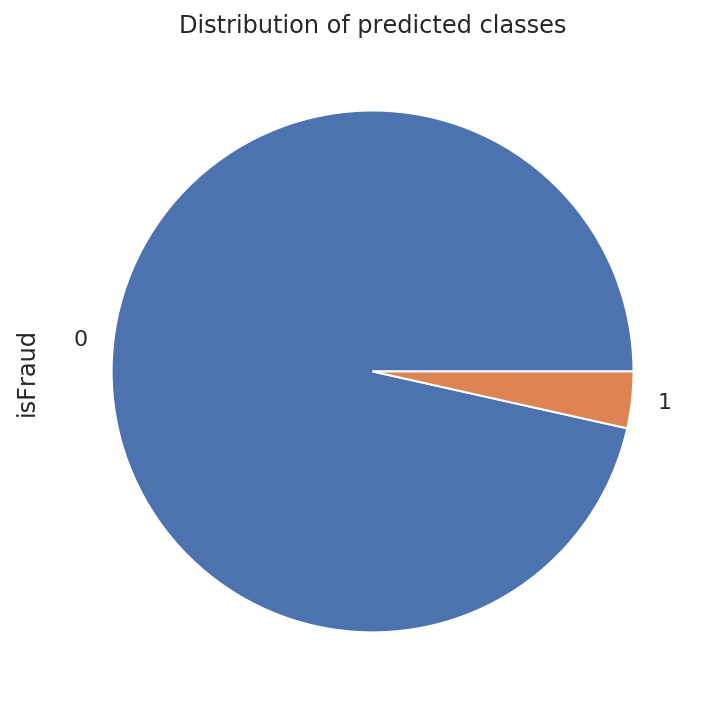
\includegraphics[width=0.5\textwidth]{figures/class_distribution.png}
    \end{center}
	\caption{Predicted classes distribution - data are highly imbalanced.}
	\label{fig:classes}
\end{figure}


\section{Method proposal}

% TODO: len kratko, co navrhujeme - feature selection na nejaky model pomocou nejakeho prirodou inspirovaneho algoritmu
% TODO: mozeno spomenut oversampling/undersampling


% usage of nature inspired algorithm proved to optimize feature selection much better than baseline well-known methods and overperforms  using power of nature inspired algorithms to address the problem of a lot of anonymized features available in existing datasets. Combination of machine learning and nature inspired algorithms proved to be the wa

% Proper data analysis in combination with training machine learning models can help to prevent frauds. Problem of choosing correct features without knowing their meaning with goal to improve detection performance can be seen as optimization problem. Nature inspired algorithms are known to be very powerful for optimization problems.


% TODO: Odôvodnenie výberu optimalizačného algoritmu
% TODO: Detailnejsia analýza hlavného algoritmu
% TODO: Návrh spôsobu nastavenia parametrov
% TODO: Návrh overenia


\section{Preparation}

Before performing experiments, we preprocessed the data. At first, useless columns like id of transaction or those with too many missing values (more than 50\%) are dropped. Our preprocessing pipeline can be devided into two branches - preprocessing of numeric and categorical attributes. In numerical attributes, missing values are filled in with mean value, then all values are normalized (some machine learning algorithms are sensitive to different scales). For categorical attributes, transformation of emails to email domains has been performed, missing values have been filled with most frequent values, small categories (smaller than 5\%) merged into one \textit{other} category and at the end, all features have been one-hot encoded. Also, missing values indicators have been added to both, numerical and categorical attributes.


% TODO: spomenut preprocessing, co sme robili a co z toho vzislo
% TODO: spomenut transformery, one hot, a filter
% TODO: kolko bol finalny pocet features
% TODO: len kratko spomenut ze preco sme sa rozhodli pouzit aky model - decision tree
% TODO: model selection phase

\section{Experiments}

We did several experiemnts in which we compared the following algorithms:

\begin{itemize}
	\item Firefly Algorithm \cite{fister2013comprehensive} - FA (alpha = 1, betamin = 1, gamma = 2)
	\item Cuckoo Search \cite{yang2009cuckoo} - CS (pa = 0.2, alpha = 0.5)
	\item Bat Algorithm \cite{yang2010new} - BA (A = 0.5, r = 0.5, Qmin = 0.0, Qmax = 2.0)
	\item Flower Pollination Algorithm \cite{yang2012flower} - FPA (p = 0.35, beta = 1.5)
	\item Grey Wolf Optimizer \cite{Mirjalili_Mirjalili_Lewis_2014} - GWO
\end{itemize}

As a baseline models we have chosen the model with all features and model with selected features from \textit{recursive feature selection with cross-validation}.

\subsection{Experiments strategy}

We chose a \textit{decision tree classifier} as a model on which we will try to find the optimal features. We kept the default hyper-parameters for this classifier set by scikit-learn library.

Since the dataset, if pretty large, firstly we \textit{undersampled} it to achieve the equal size of both classes. Then we shrunk it again to 5\% of its size, so we would be able to make as many experiments as possible (we did not have enough computing power). We did a train/test split of 80/20.

For each algorithm, we tried several population sizes (10, 20, and 50), for which we did 5 runs of the algorithm. We trained exactly 50 generations. For both, recursive feature selection and feature selection using nature-inspired algorithms we did 5 fold cross-validation. We did not experiment with algorithm parameters and we used their defaults which are described in the previous section.

\subsection{Results}

When comparing the population sizes, all of the algorithms achieved the best results when the population size was highest (50). The only exception is Cuckoo Search, which found the most optimal solution with population size 10, however the difference negligible. Table \ref{tab:nia_comparison}. shows the algorithm scores for each population. Figure \ref{fig:nia_train_score_by_algorithm}. shows the differences in scores between population size of 10 and 50.

\begin{figure}
    \centering
    \subfloat{{ 
        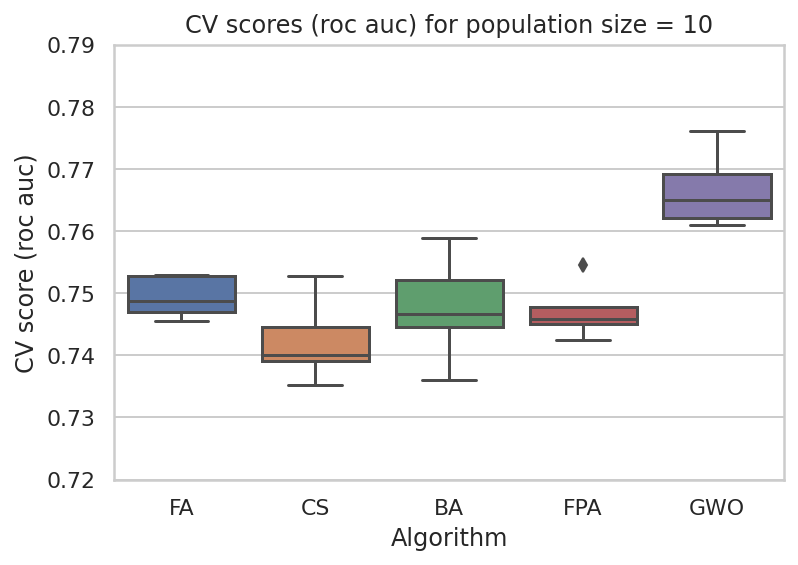
\includegraphics[width=5.5cm]{figures/nia_train_score_by_algorithm_10}
    }}
    \qquad
    \subfloat{{
        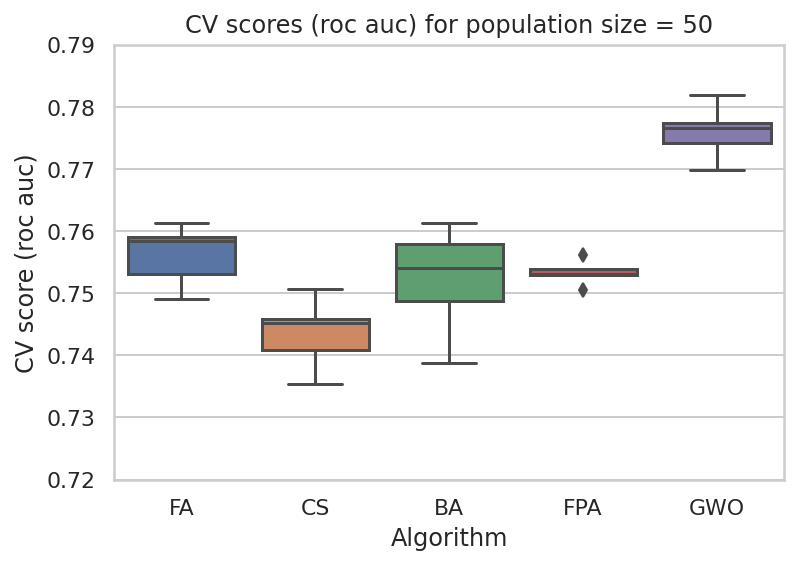
\includegraphics[width=5.5cm]{figures/nia_train_score_by_algorithm_50}
    }}
    \caption{Scores of the algorithms by the population size. The scores are slightly higher for population size of 50.}
    \label{fig:nia_train_score_by_algorithm}
\end{figure}

\begin{table}[]
	\begin{center}
		\begin{tabular}{|l|rrrrr|}
			\hline
			\textbf{Population size \textbackslash Score} & \multicolumn{1}{l}{\textbf{FA}} & \multicolumn{1}{l}{\textbf{CS}} & \multicolumn{1}{l}{\textbf{BA}} & \multicolumn{1}{l}{\textbf{FPA}} & \multicolumn{1}{l|}{\textbf{GWO}} \\ \hline
			\textbf{10}                                             & 0.753                           & \textbf{0.752}                           & 0.759                           & 0.754                            & 0.776                             \\
			\textbf{20}                                             & 0.757                           & 0.746                           & 0.755                           & 0.750                            & 0.771                             \\
			\textbf{50}                                             & \textbf{0.761}                           & 0.751                           & \textbf{0.761}                           & \textbf{0.756}                            & \textbf{0.782}                             \\ \hline
		\end{tabular}
	\end{center}
	\begin{center}
		\caption{Highest train scores (ROC AUC) of nature inspired algorithms by population size. We may notice that Grey Wolf Algorithm (GWO) outperformed all of the other algorithms.} \label{tab:nia_comparison}
	\end{center}
\end{table}

All of the nature-inspired algorithms perform roughly the same, except the Grey Wolf Optimizer which outperformed the others (Figure \ref{fig:nia_train_score_by_algorithm}). These differences in results (means) between GWO and other algorithms are significant (t-test; $p-value=0.012$). Looking for the explanation, we found out that only Grey Wolf Algorithm and Bat Algorithm converged during the optimization run. Figure \ref{fig:nia_scores_by_run} shows the optimization of the Firefly Algorithm and Grey Wolf Optimizer, the difference is noticeable. If we fine-tuned the parameters of other algorithms, they might converge as well. The fact that GWO does not have any parameters (except the population size) was an advantage for it in our experiments.

% https://towardsdatascience.com/hypothesis-testing-in-machine-learning-using-python-a0dc89e169ce

\begin{figure}
    \centering
    \subfloat[Firefly Algorithm]{{ 
        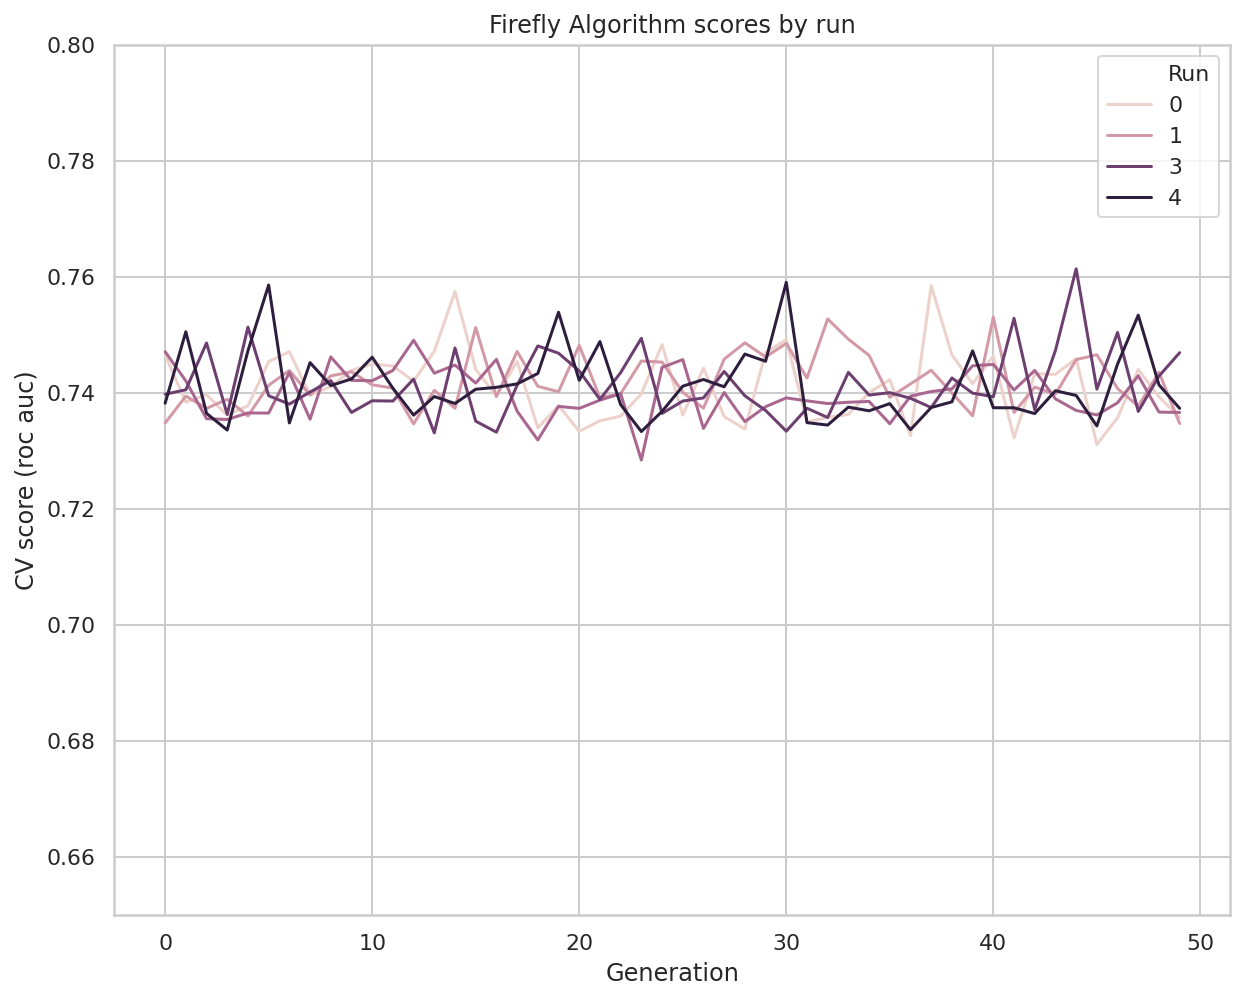
\includegraphics[width=5.5cm]{figures/fa_scores_by_run}
    }}
    \qquad
    \subfloat[Grey Wolf Optimizer]{{
        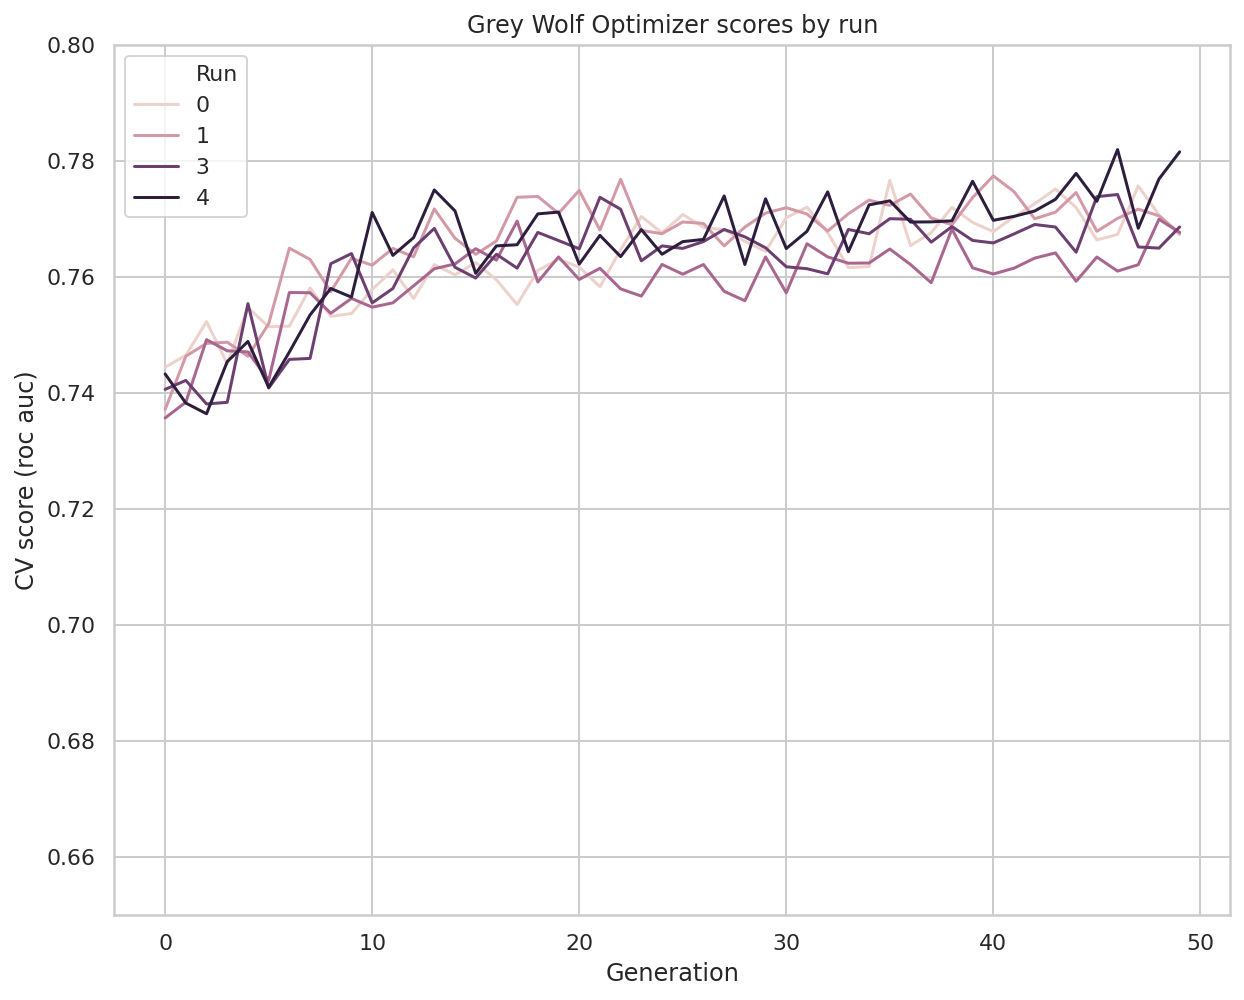
\includegraphics[width=5.5cm]{figures/gwo_scores_by_run}
    }}
    \caption{Optimization progress for 5 runs of Grey Wolf Optimizer and Firefly Algorithm. The Firefly Algorithm did not really converge.}
    \label{fig:nia_scores_by_run}
\end{figure}

The best features, selected by the optimization process, were later used to train the final model on test data. These models were compared to a model trained on all features and the model trained on features selected by recursive feature elimination.

The nature-inspired algorithms found a more optimal set of features on the train dataset than recursive feature elimination. However, they achieved worse results on the test dataset. The only exception is Grey Wolf Optimizer, which achieved the best train and test score. The most noticeable difference in the results is the number of selected features by algorithms. All of the algorithms (including recursive feature elimination), selected around $~110$ features, however, GWO selected only 53, this is probably the reason of its results. These results are shown in Table \ref{tab:nia_baseline_comparison}. Figure \ref{fig:nia_selected_features_by_algorithm} shows that GWO selected fewer features in general not only in its best solution.

\begin{table}[]
	\begin{center}
		\begin{tabular}{|lrrr|}
			\hline
			\textbf{Feature selection type} & \textbf{Train score} & \textbf{Test score} & \textbf{Selected features} \\ \hline
			All features                    & N/A                  & 0.713               & 240                                  \\
			Recursive feature elimination   & 0.747                & 0.719               & 112                                  \\
			Firefly Algorithm               & 0.761                & 0.663               & 114                                  \\
			Cuckoo Search                   & 0.753                & 0.718               & 106                                  \\
			Bat Algorithm                   & 0.761                & 0.689               & 125                                  \\
			Flower Pollination Algorithm    & 0.756                & 0.706               & 113                                  \\
			\textbf{Grey Wolf Optimizer}             & \textbf{0.782}                & \textbf{0.733}               & \textbf{53}                                   \\ \hline
		\end{tabular}
	\end{center}
	\begin{center}
		\caption{Comparison of the baseline models with nature-inspired algorithms. The train score stands for the best score from the optimization. All of the nature-inspired algorithms (except Grey Wolf Optimizer) achieved a better train score than recursive feature elimination, however, they overfit the model which resulted in a worse test scores.} \label{tab:nia_baseline_comparison}
	\end{center}
\end{table}

\begin{figure}[ht]
	\begin{center}
	    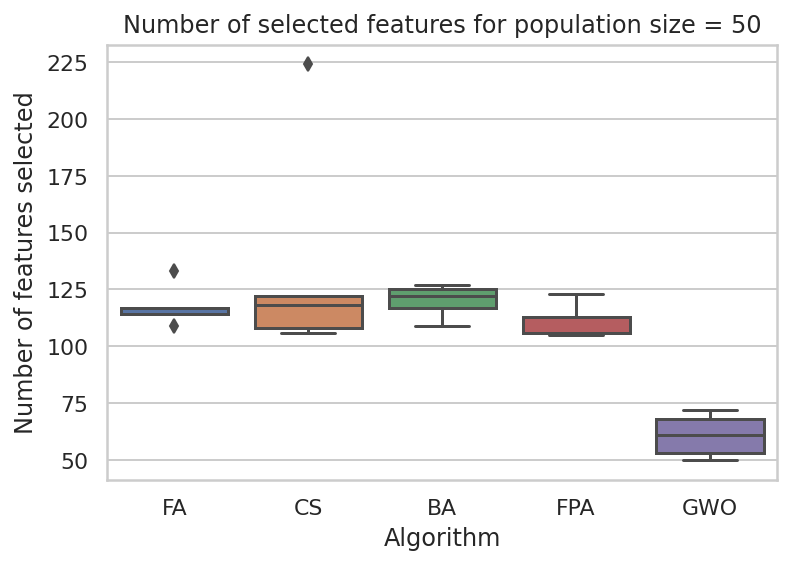
\includegraphics[width=5.5cm]{figures/nia_selected_features_by_algorithm.png}
    \end{center}
	\caption{Number of selected features by algorithm - Grey Wolf Algorithm selected by far the least number of features.}
	\label{fig:nia_selected_features_by_algorithm}
\end{figure}

% TODO: ake experiemnty sme spravili
% TODO: tabulka porovnania algoritmov
% TODO: learning along the way with consequences - napr undersampling/oversampling atd.

\section{Conclusion}

% TODO: zhrnutie vysledkov, mozne vylepsenia a uskalia nasho pristupu

In our experiments, we found out Grey Wolf Optimizer as the best nature-inspired algorithm for feature selection. It achieved significantly better results than other nature-inspired algorithms and better results that recursive feature elimination.

GWO alongside Bat Algorithm was the only nature-inspired algorithms that were able to converge during the optimization process. We assume that other algorithms might converge too if we experimented with their parameter settings. We consider the fact, that GWO does not have any parameters other than population size as a big strength, because it saves a significant amount of optimization time.

In comparison with traditional ways of feature selection (recursive feature elimination), all of the nature-inspired algorithms were able to find better solutions on the training dataset, however, they overfit most of the time. Moreover, the feature selection using nature-inspired algorithms was much slower.

\bibliographystyle{splncs04}
\bibliography{references}

\end{document}
